\documentclass{../../slides-style}

\slidetitleext{Лекция 6/Практика 5: Структурные шаблоны}{17.04.2025}{Структурные шаблоны}

\begin{document}

    \begin{frame}[plain]
        \titlepage
    \end{frame}

    \section{Введение}

    \begin{frame}
        \frametitle{Паттерны проектирования}
        \textbf{Шаблон проектирования} --- это повторимая архитектурная конструкция, являющаяся решением некоторой типичной технической проблемы
        \begin{itemize}
            \item Подходит для класса проблем
            \item Обеспечивает переиспользуемость знаний
            \item Позволяет унифицировать терминологию
            \item В удобной для изучения форме
            \item НЕ конкретный рецепт или указания к действию
        \end{itemize}
    \end{frame}

    \begin{frame}
        \frametitle{Паттерны и архитектурные стили}
        \begin{center}
            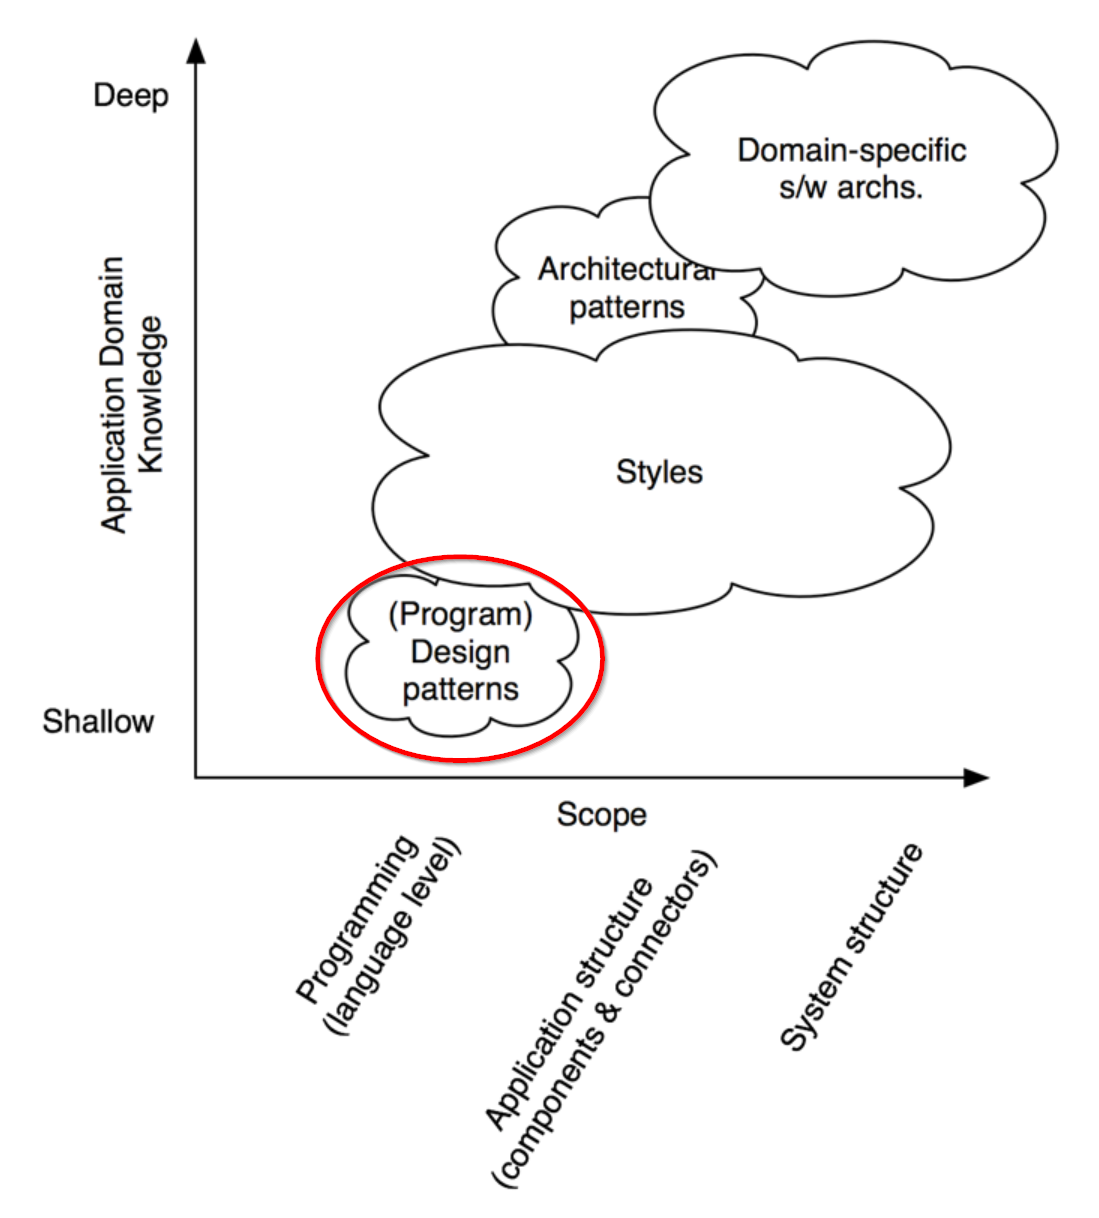
\includegraphics[width=0.5\textwidth]{architecturalStylesPatternsHighlighted.png}
            \attribution{N. Medvidovic}
        \end{center}
    \end{frame}

    \begin{frame}
        \frametitle{Книжка про паттерны}
        \framesubtitle{Must read!}

        \begin{columns}
            \begin{column}{0.6\textwidth}
                Приемы объектно-ориентированного проектирования. Паттерны проектирования

                Э. Гамма, Р. Хелм, Р. Джонсон, Дж. Влиссидес

                Design Patterns: Elements of Reusable Object-Oriented Software
            \end{column}
            \begin{column}{0.4\textwidth}
                \begin{center}
                    
\includegraphics[width=0.8\textwidth]{patternBookCover.png}
                \end{center}
            \end{column}
        \end{columns}
    \end{frame}

    \section{Модельный пример}

    \begin{frame}
        \frametitle{Начнём с примера}
        \framesubtitle{Текстовый редактор}
        WYSIWYG-редактор, основные вопросы:
        \begin{itemize}
            \item Структура документа
            \item Форматирование
            \item Создание привлекательного интерфейса пользователя
            \item Поддержка стандартов внешнего облика программы
            \item Операции пользователя, undo/redo
            \item Проверка правописания и расстановка переносов
        \end{itemize}
    \end{frame}

    \section{Паттерн ``Декоратор''}

    \begin{frame}
        \frametitle{Усовершенствование UI}
        \begin{itemize}
            \item Хотим сделать рамку вокруг текста и полосы прокрутки, отключаемые по опции
            \item Желательно убирать и добавлять элементы обрамления так, чтобы другие объекты даже не знали, что они есть
            \item Хотим менять во время выполнения --- наследование не подойдёт
            \begin{itemize}
                \item Наш выбор ­--- композиция
                \item Прозрачное обрамление
            \end{itemize}
        \end{itemize}
    \end{frame}

    \begin{frame}
        \frametitle{Моноглиф}
        \begin{columns}
            \begin{column}{0.6\textwidth}
                \begin{itemize}
                    \item Абстрактный класс с ровно одним сыном
                    \begin{itemize}
                        \item Вырожденный случай компоновщика
                    \end{itemize}
                    \item ``Обрамляет'' сына, добавляя новую функциональность
                \end{itemize}
            \end{column}
            \begin{column}{0.4\textwidth}
                \begin{center}
                    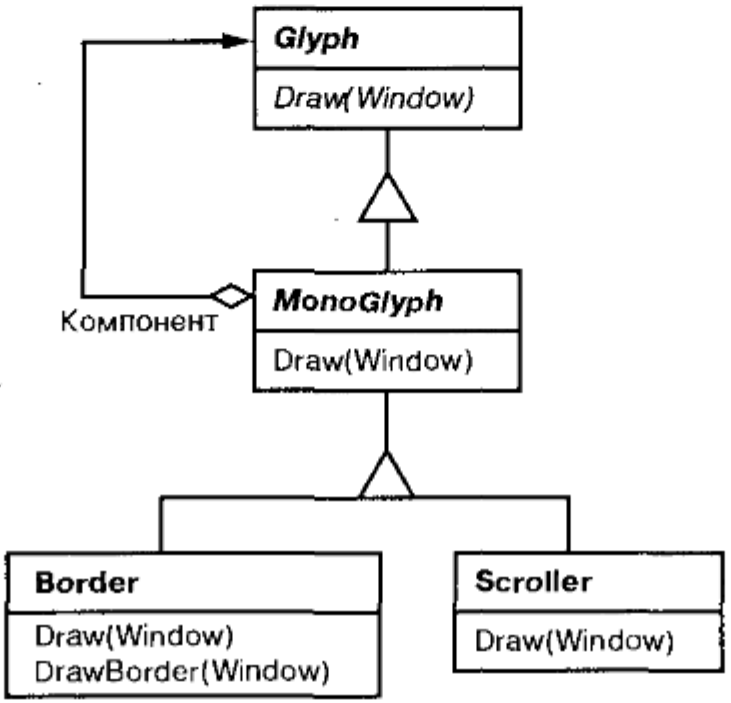
\includegraphics[width=0.9\textwidth]{monoglyph.png}
                    \attribution{Э. Гамма и др., Приемы объектно-ориентированного проектирования}
                \end{center}
            \end{column}
        \end{columns}
    \end{frame}

    \begin{frame}
        \frametitle{Структура глифов}
        \begin{center}
            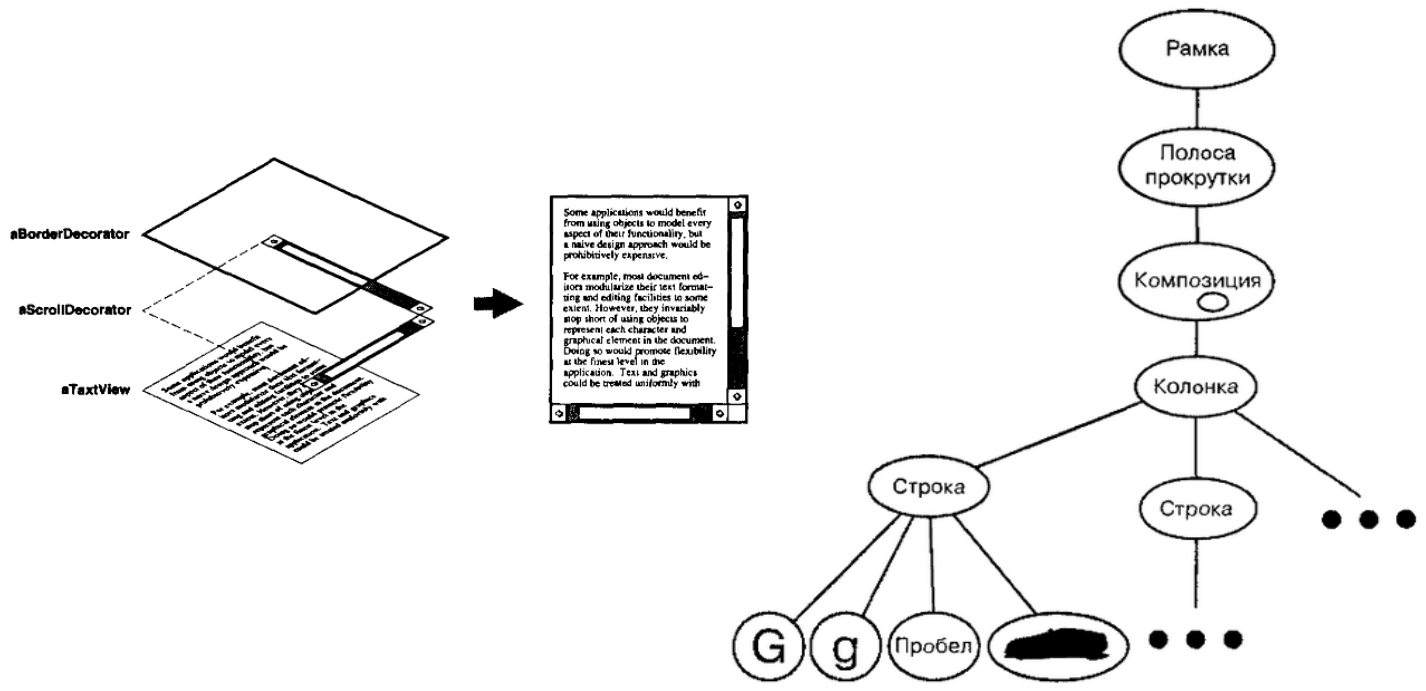
\includegraphics[width=0.9\textwidth]{glyphStructure.png}
            \attribution{Э. Гамма и др., Приемы объектно-ориентированного проектирования}
        \end{center}
    \end{frame}

    \begin{frame}
        \frametitle{Паттерн ``Декоратор''}
        \framesubtitle{Decorator}
        \begin{center}
            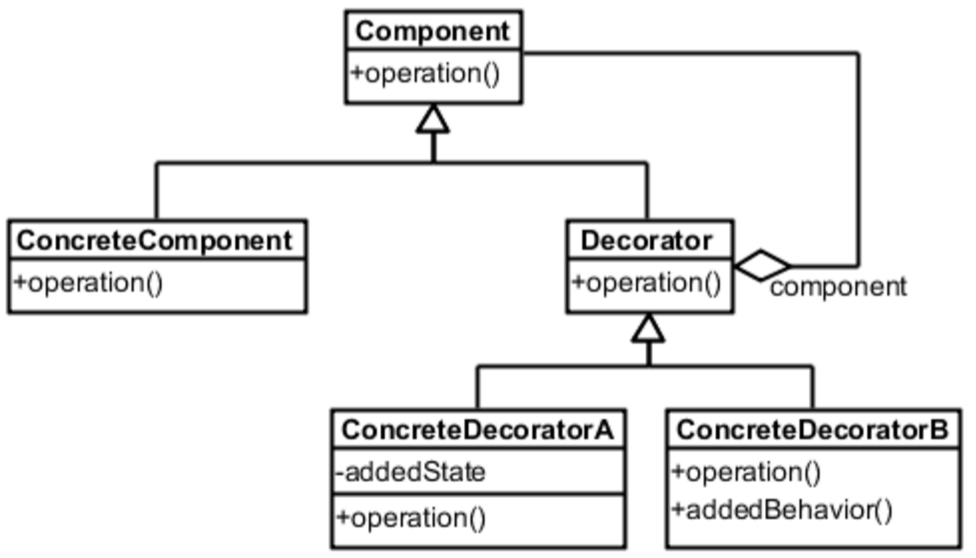
\includegraphics[width=0.6\textwidth]{decorator.png}
        \end{center}
    \end{frame}

    \begin{frame}
        \frametitle{Декоратор, особенности}
        \begin{itemize}
            \item Динамическое добавление (и удаление) обязанностей объектов
            \begin{itemize}
                \item Большая гибкость, чем у наследования
            \end{itemize}
            \item Позволяет избежать перегруженных функциональностью базовых классов
            \item Много мелких объектов
        \end{itemize}
    \end{frame}

    \begin{frame}
        \frametitle{``Декоратор'' (Decorator), детали реализации}
        \begin{columns}
            \begin{column}{0.6\textwidth}
                \begin{itemize}
                    \item Интерфейс декоратора должен соответствовать интерфейсу декорируемого объекта
                    \begin{itemize}
                        \item Иначе получится ``Адаптер''
                    \end{itemize}
                    \item Если конкретный декоратор один, абстрактный класс можно не делать
                \end{itemize}
            \end{column}
            \begin{column}{0.4\textwidth}
                \begin{center}
                    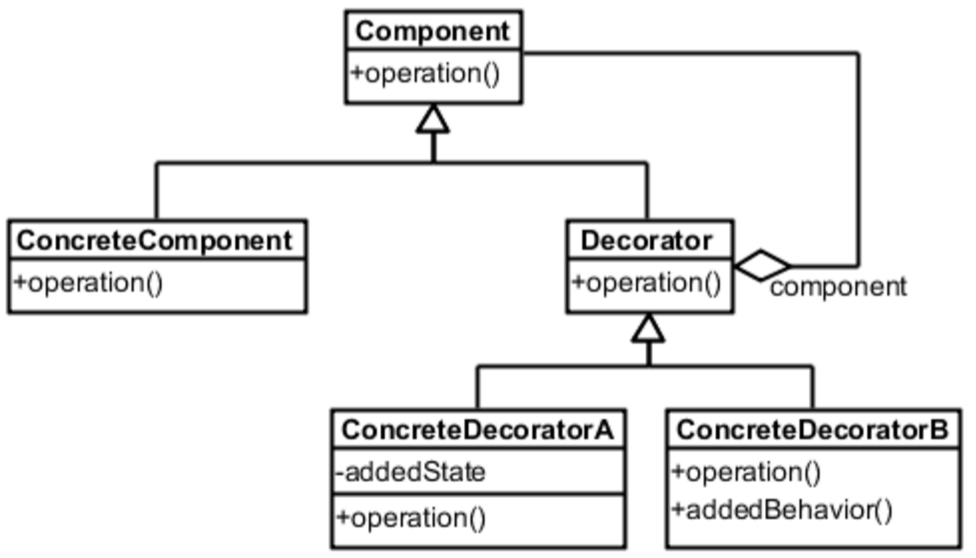
\includegraphics[width=\textwidth]{decorator.png}
                \end{center}
            \end{column}
        \end{columns}
        \begin{itemize}
            \item Component должен быть по возможности небольшим (в идеале, интерфейсом)
            \begin{itemize}
                \item Иначе лучше паттерн ``Стратегия''
                \item Или самодельный аналог, например, список ``расширений'', которые вызываются декорируемым объектом вручную перед операцией или после неё
            \end{itemize}
        \end{itemize}
    \end{frame}

    \section{Паттерн ``Стратегия''}

    \begin{frame}
        \frametitle{Форматирование текста}
        \begin{itemize}
            \item Задача --- разбиение текста на строки, колонки и т.д.
            \item Высокоуровневые параметры форматирования
            \begin{itemize}
                \item Ширина полей, размер отступа, межстрочный интервал и т.д.
            \end{itemize}
            \item Компромисс между качеством и скоростью работы
            \item Инкапсуляция алгоритма
        \end{itemize}
    \end{frame}

    \begin{frame}
        \frametitle{Compositor и Composition}
        \begin{center}
            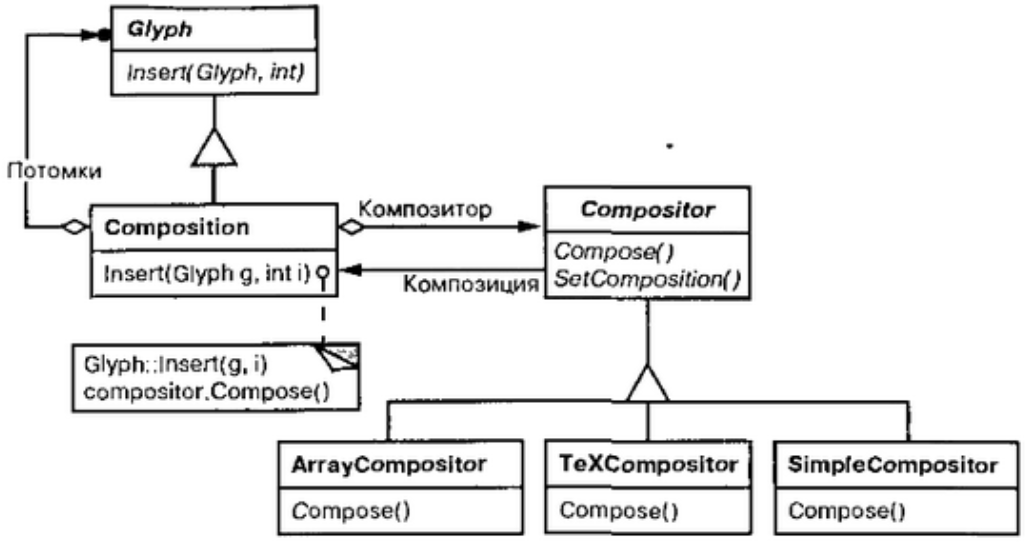
\includegraphics[width=0.7\textwidth]{compositor.png}
            \attribution{Э. Гамма и др., Приемы объектно-ориентированного проектирования}
        \end{center}
    \end{frame}

    \begin{frame}
        \frametitle{Паттерн ``Стратегия''}
        \framesubtitle{Strategy}
        \begin{itemize}
            \item Назначение --- инкапсуляция алгоритма в объект
            \item Самое важное --- спроектировать интерфейсы стратегии и контекста
            \begin{itemize}
                \item Так, чтобы не менять их для каждой стратегии
            \end{itemize}
            \item Применяется, если
            \begin{itemize}
                \item Имеется много родственных классов с разным поведением
                \item Нужно иметь несколько вариантов алгоритма
                \item В алгоритме есть данные, про которые клиенту знать не надо
                \item В коде много условных операторов
            \end{itemize}
        \end{itemize}
        \begin{center}
            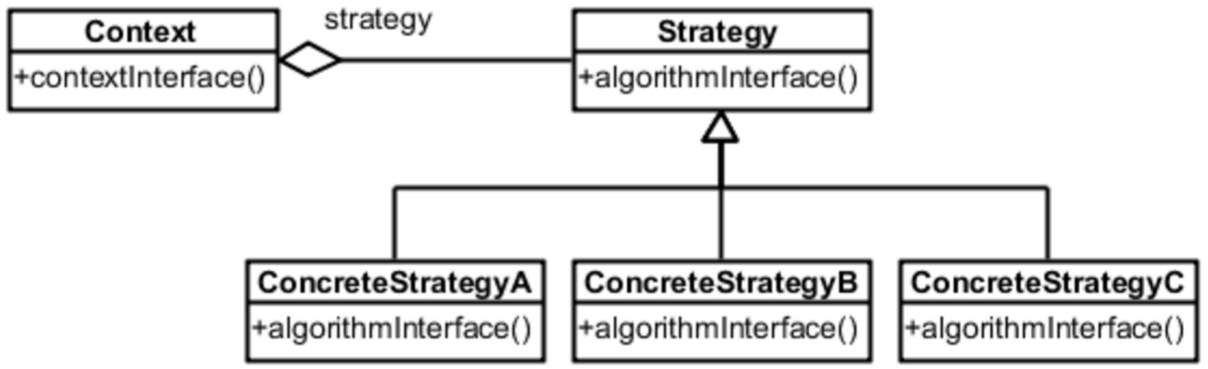
\includegraphics[width=0.6\textwidth]{strategy.png}
        \end{center}
    \end{frame}

    \begin{frame}
        \frametitle{``Стратегия'' (Strategy), детали реализации}
        \begin{center}
            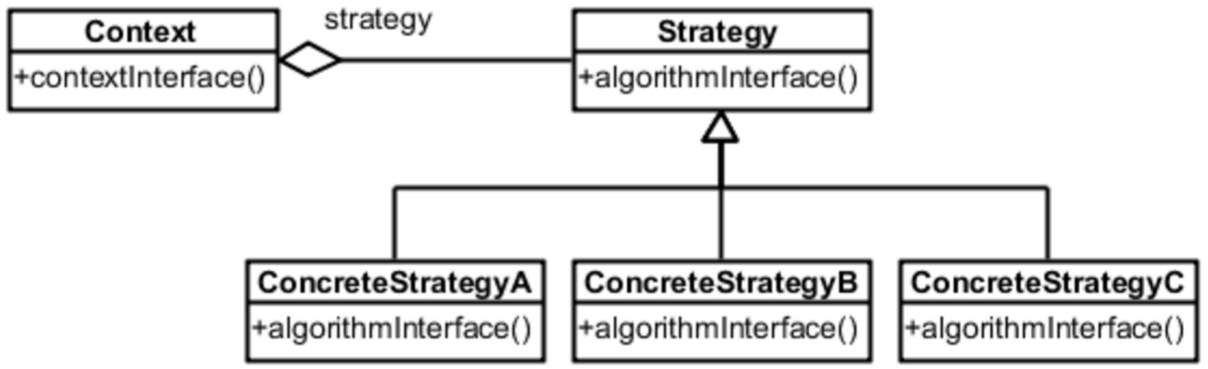
\includegraphics[width=0.6\textwidth]{strategy.png}
        \end{center}
        \begin{itemize}
            \item Передача контекста вычислений в стратегию
            \begin{itemize}
                \item Как параметры метода --- уменьшает связность, но некоторые параметры могут быть стратегии не нужны
                \item Передавать сам контекст в качестве аргумента --- в Context интерфейс для доступа к данным
            \end{itemize}
        \end{itemize}
    \end{frame}

    \begin{frame}
        \frametitle{``Стратегия'' (Strategy), детали реализации (2)}
        \begin{itemize}
            \item Стратегия может быть параметром шаблона
            \begin{itemize}
                \item Если не надо её менять на лету
                \item Не надо абстрактного класса и нет оверхеда на вызов виртуальных методов
            \end{itemize}
            \item Стратегия по умолчанию
            \begin{itemize}
                \item Или просто поведение по умолчанию, если стратегия не установлена
            \end{itemize}
            \item Объект-стратегия может быть приспособленцем
        \end{itemize}
    \end{frame}

    \section{Задание на практику}

    \begin{frame}
        \frametitle{Задачи на дом}
        Уточнить модель компьютерной игры Roguelike с предыдущего занятия:

        \begin{enumerate}
            \item Используя шаблон ``Стратегия'' для поддержки различных поведений мобов
            \begin{itemize}
                \item Агрессивное поведение, атакуют игрока, как только его видят
                \item Пассивное поведение, просто стоят на месте
                \item Трусливое поведение, стараются держаться на расстоянии от игрока
            \end{itemize}
            \item Используя шаблон ``Декоратор'' для поддержки временных эффектов, накладываемых на мобов и игрока
            \begin{itemize}
                \item Эффект конфузии, заставляющий персонажа двигаться в случайном направлении
                \item Возможность добавить другие похожие эффекты
            \end{itemize}
        \end{enumerate}
    \end{frame}

\end{document}
